\begin{prob}[4]\textbf{Feasibility of an LP:}
\end{prob}
 Develop an algorithm to test the feasiblity of an
  LP using the approach in (11.19) where $f_{i}(x)$ are affine functions
  of $x$. Express the gradients and the Hessians needed for the algorithm
  explicitly in your report and describe the algorithm.

OBJECTIVE FUNCTION
\begin{eqnarray*}
\mbox{minimize } s\\
\mbox{subject to } Ax - b \preccurlyeq \mathbf{1} s
\end{eqnarray*}
where $x \in \mathbf{R^{n}}$, $s \in \mathbf{R}$, $x \in \mathbf{R^{m \times n}}$, and  $b \in \mathbf{R^{m}}$.\\
For a basic phase I optimization problem, the problem must be restated in log-barrier form as follows:
\[
\mbox{minimize } ts - \sum \log [\mathbf{1}s + b - Ax]
\]
where $t \in \mathbf{R}$ is a scalar value used in the barrier method.

GRADIENT OF OBJECTIVE FUNCTION
\[
\nabla f(x, s) = \begin{bmatrix}
\dfrac{\partial f(x, s)}{\partial x}\\
\dfrac{\partial f(x, s)}{\partial s}
\end{bmatrix}
\]
where:
\begin{eqnarray*}
\dfrac{\partial f(x, s)}{\partial x} &= \dfrac{A^{T}}{\mathbf{1}s + b - Ax}\\
\dfrac{\partial f(x, s)}{\partial s} &= t - \sum \dfrac{1}{\mathbf{1}s + b - Ax}\\
\end{eqnarray*}

HESSIAN OF OBJECTIVE FUNCTION
\[
\nabla^{2} f(x, s) = \begin{bmatrix}
\dfrac{\partial^{2} f(x, s)}{\partial x^{2}} & \dfrac{\partial^{2} f(x, s)}{\partial x \partial s}\\
\dfrac{\partial^{2} f(x, s)}{\partial s \partial x} & \dfrac{\partial^{2} f(x, s)}{\partial s^{2}}
\end{bmatrix}
\]
where:
\begin{eqnarray*}
\dfrac{\partial^{2} f(x, s)}{\partial x^{2}} &=& \begin{cases}
\dfrac{a^{2}_{ij}}{\mathbf{1}s + b - Ax^{2}} & \mbox{if } i = j\\
\dfrac{\prod_{j=1}^{n}a_{ij}}{\mathbf{1}s + b - Ax} & \mbox{otherwise}
\end{cases}\\ 
\dfrac{\partial^{2} f(x, s)}{\partial x \partial s} &=& \dfrac{-A^{T}}{\mathbf{1}s + b - Ax^{2}}\\
\dfrac{\partial^{2} f(x, s)}{\partial s \partial x} &=& \dfrac{-A^{T}}{\mathbf{1}s + b - Ax^{2}}\\
\dfrac{\partial^{2} f(x, s)}{\partial s^{2}} &=& \sum_{i=1}^{m} \dfrac{1}{\mathbf{1}s + b - Ax^{2}}
\end{eqnarray*}

  \begin{figure}[ht]
  \centering
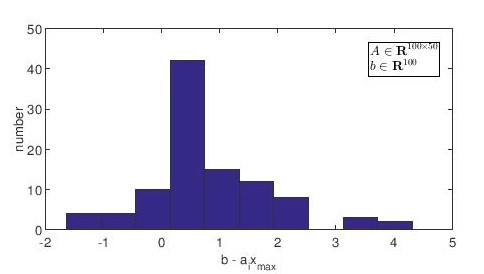
\includegraphics[width=7cm]{source/prob4/fig1}
%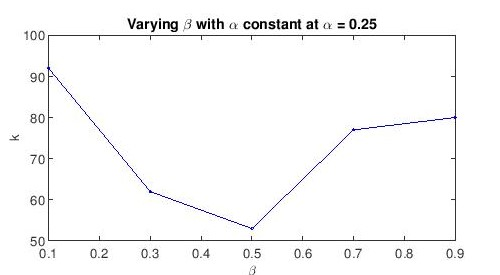
\includegraphics[width=5cm]{source/prob1/fig4}
\caption{Distribution of $b_{i} - a_{i} x_{max}$ for a set of inequalitites $A x \preccurlyeq b$ where $A \in \mathbf{R^{100 \times 50}}$ and $ b \in \mathbf{R^{100}}$}
\end{figure}

EFFECT OF $\mu$

For small $\mu$, the barrier method parameter $t$ increases by a small amount in each iteration; so, the iterations are fairly close to each other, and tend to the central path.

For large $\mu$, the barrier method parameter $t$ increases by a large amount; so, each iteration is not a good approximation of the next iteration. This means that we would require more Newton Method iterations to minimize the log-barrier optimization function.